\chapter{Experiments}

We evaluate our software for isometric reconciliation on a simulated and real dataset that were used to evaluate SPIMAP \cite{spimap} and TreeFix \cite{treefix} in previous studies. The simulated dataset consists of 1000 simulated gene families of two clades of species: 12 \emph{Drosophila} genomes and 16 fungal genomes, generated with the SPIMAP model. The real dataset includes 5351 real gene families from 16 fungal genomes.

To compare, we run other software for computing the gene tree reconciliation: Notung \cite{notung}, TreeFix \cite{treefix} and Treerecs \cite{treerecs}, on the same dataset.

\section{Simulated dataset}

In the simulated dataset, we know the correct gene tree with its evolutionary events, which allows us to test several aspects. In the experiments, we measure the accuracy of correctly inferred topology, branches, duplications and gene losses. For each software, we measure the time of computing the results. 

We evaluate our software for isometric reconciliation for two cases: a rooted gene tree with different tolerance settings and an unrooted gene tree with different step and tolerance setting. In the first case, we take the rooted gene tree as it is from the dataset and run a reconciliation with \emph{countDL} function (Algorithm \ref{countDL} in Chapter \ref{main_algorithm}). We evaluate it several times with different tolerance setting to scale up the edges. The tolerance setting are $0.0, 0.000001, 0.00001, 0.001, 0.1, 0.3, 0.5, 1.0$ and the $\epsilon = \num{1e-6}$.

The second case takes the rooted gene tree as input with an argument to reroot the given gene tree. We forget the root of the rooted gene tree and transform it into the unrooted gene tree. On the obtained unrooted gene tree, we run the \emph{getIntervals} function (Algorithm \ref{getIntervals} in Chapter \ref{rooting_the_gene_tree}) to subdivide each edge of the unrooted gene tree and then run a reconciliation with \emph{countDL} function (Algorithm \ref{countDL} in Chapter \ref{main_algorithm}). We want to find a new root minimizing the number of inferred duplications and gene losses in reconciliation. The process is executed several times with different tolerance and step settings. The tolerance and $\epsilon$ setting are the same as in the first case. The step setting are $0.0, 0.3, 0.5, 1.0, 2.0$.

\section{Real dataset}

%ako sme spracovali align
The correct gene tree is unknown in the real dataset, thus we use different metrics as with the simulated dataset. We measure the number of inferred duplications and gene losses overall gene trees in the dataset and the consistency score of duplications.

The duplication consistency score $dcs$ shows the plausibility of inferred duplications. For a duplication node $u$ with children $v$ and $w$, the duplication consistency score $dcs(u) = (L \cup R) \mid (L \cap R)$ is computed as the union of $L$ and $R$ over intersection of $L$ and $R$, where $L$ is the set of species represented in left child $v$ and $R$ is the set of species represented in right child $w$.

\begin{figure}[ht!]
	\centering
	\label{consistency_score}
  	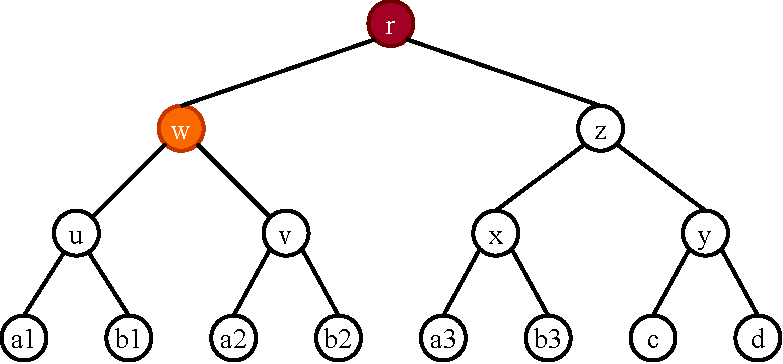
\includegraphics[width=\linewidth]{consistency_score}
  	\caption[Duplication consistency score]{\textbf{Duplication consistency score for node $w$}\\
  	The set of species of left child $u$ is $L = \{A, B\}$ and the set of species of right child $v$ is $R = \{A, B\}$. The duplication consistency score is computed as: $dcs(w) = (L \cup R) \mid (L \cap R) = 2 \div 2 = 1$.
  	\\
  	\textbf{Duplication consistency score for node $r$}\\
  	The set of species of left child $w$ is $L = \{A, B\}$ and the set of species of right child $z$ is $R = \{A, B, C, D\}$. The duplication consistency score is computed as: $dcs(r) = (L \cup R) \mid (L \cap R) = 2 \div 4 = 0.5$.}
\end{figure}

